\chapter{Comparaison avec un cas de la littérature}
L'objectif de cette partie est de comparer les résultats obtenus par TrioCFD avec ceux présentés par Rao et al. \cite{rao_influence_2015}. Dans leur article Rao et al. présentent une expérience ainsi qu'un modèle CFD associé à l'experience permettant de modéliser le transfert de masse pour un cas ternaire.
\section{Présentation du cas de référence}
L'objectif de l'expérience est de visualiser la diffusion dans de l'eau de l'acétonitrile (miscible) contenue initialement dans une goutte composée également de chlorobenzène (non miscible). Ainsi à l'instant initial une goutte contenant un mélange d'acétonitrile et de chlorobenzène est formée, cette dernière étant plus légère que l'eau dans laquelle elle se trouve va commencer à monter, puis sous l'effet de la diffusion massique un changement de rapport de densité va subvenir et la goutte va redescendre.  
\begin{figure}[H]
	\centering
	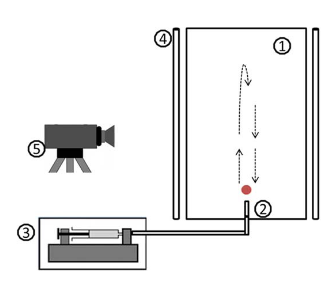
\includegraphics[width=0.3\linewidth]{figure/exp}
	\caption{Schéma de l'expérience, d'après \cite{rao_influence_2015}}
	\label{fig:exp}
\end{figure}
L'article présente également un modèle CFD, dans celui-ci le transfert de masse est calculé semi-empiriquement, à chaque itération la position de la goutte obtenue numériquement est comparée à la position obtenue expérimentalement, puis une régulation est mise en place pour déterminer un coefficient de transfert de masse via des corrélations pour faire diminuer cet écart, le ”modèle” alors obtenu n’est pas prédictible et une expérience physique est toujours nécessaire pour réaliser une simulation. L'algorithme est présenté en figure \ref{fig:algoRao}, 
\begin{figure}[H]
	\centering
	\begin{tikzpicture}[scale=0.75, transform shape]
	\node[draw,aspect=1.3, text centered,text width=3cm] (V) at (0,2.3) {Solution initiale };
	\node[draw,aspect=1.3, text centered,text width=2cm] (T) at (0,1.3) {$n=n+1$ };
	\node[draw,rectangle, text centered,minimum width=2cm,minimum height=1cm] (A)at(0,0){Estimation du transfert de masse à partir de corrélations};
	\node[draw,text centered,minimum width=2cm,minimum height=1cm] (B) at (0,-1.5) {Résolution des équations de Navier-Stokes};
	\node[draw,text centered,text width=10cm,minimum height=1cm] (C) at (0,-3) {Comparaison entre l'altitude de la goutte obtenue par CFD avec l'expérience, res = $f(z_{\text{CFD}},z_{\text{exp}})$};
	\node[draw,rectangle,diamond, aspect=1.3, text centered,text width=1.5cm] (D) at (0,-5) {res $<\varepsilon$ ? };
	
	\node[draw,rectangle,diamond, aspect=1.3, text centered,text width=1.5cm] (E) at (0,-7.3
	) { $t^{f}<t^{n}$ ? };
	\node[draw,aspect=1.3, text centered,text width=1.5cm] (W) at (0,-9) {Fin};
	%\node[draw,text centered,text width=2cm,minimum height=1cm] (E) at (0,-6.8) { $t=t^{n+1}$};
	%\node[draw,text centered,text width=7cm,minimum height=1cm] (Z) at (0,-6.2) { dsq}
	
	\node[draw,rectangle,diamond, aspect=1.3, text centered,text width=1cm,color=white] (H)at(-5,-5.9){ };
	\node[text centered,text width=1cm,color=black] (K1)at(0.5,-5.9){oui};
	\node[text centered,text width=1cm,color=black] (K2)at(-1.5,-4.8){non};
	\node[text centered,text width=1cm,color=black] (K3)at(0.5,-8.3){oui};
	\node[text centered,text width=1cm,color=black] (K4)at(-1.5,-7){non};
	%\node[draw,rectangle, text centered,diamond, aspect=1.3, text centered,text width=1cm] (I)at(6,-6){i=1 to n-1};
	\draw[->] (T.south) -- (A.north);
	\draw[->] (A.south) -- (B.north);
	\draw[->] (B.south) -- (C.north);
	\draw[->] (C.south) -- (D.north);
	\draw[->] (D.south) -- (E.north);
	\draw[->] (V.south) -- (T.north);
	\draw[->] (E.south) -- (W.north);
	\draw[->] (-7,1.3) -- (T.west);
	
	
	
	\draw (D.west)-- (-6,-5);
	\draw (-6,-5)-- (-6.,0);
	%	\draw (F.west)-- (-6.,0);
	\draw[->] (-6.,0) -- (A.west);
	\draw[-] (E.west) -- (-7,-7.3);
	\draw[-] (-7,-7.3) -- (-7,1.3);
	%\draw (G.east)-| (I.south);
	%\draw[->] (I.north)|- (A.east);
	\end{tikzpicture}
	\caption{Algorithme de résolution développé par Rao et al.\cite{rao_influence_2015}}
	\label{fig:algoRao}
\end{figure}
\section{Simulation réalisées}
\subsection{Choix du paysage thermodynamique}
L'objectif est alors d'utiliser un paysage de ce type pour résoudre un problème donné, pour cela quelques règles sont à garder en tête pour le choix d'un paysage thermodynamique. Dans un premier temps il est essentiel que les conditions initiales ne soient pas incluse dans la lacune de miscibilité, ce qui entraînerait une séparation de phase immédiate, un exemple de paysage de ce type est donnée en figure \ref{fig:landscapebase} et les résultats sont présentés par la figure \ref{land_base_sep}, on y observe une séparation de phase dès les premiers instants du calcul .
 \begin{figure}[H]
 	\centering
 	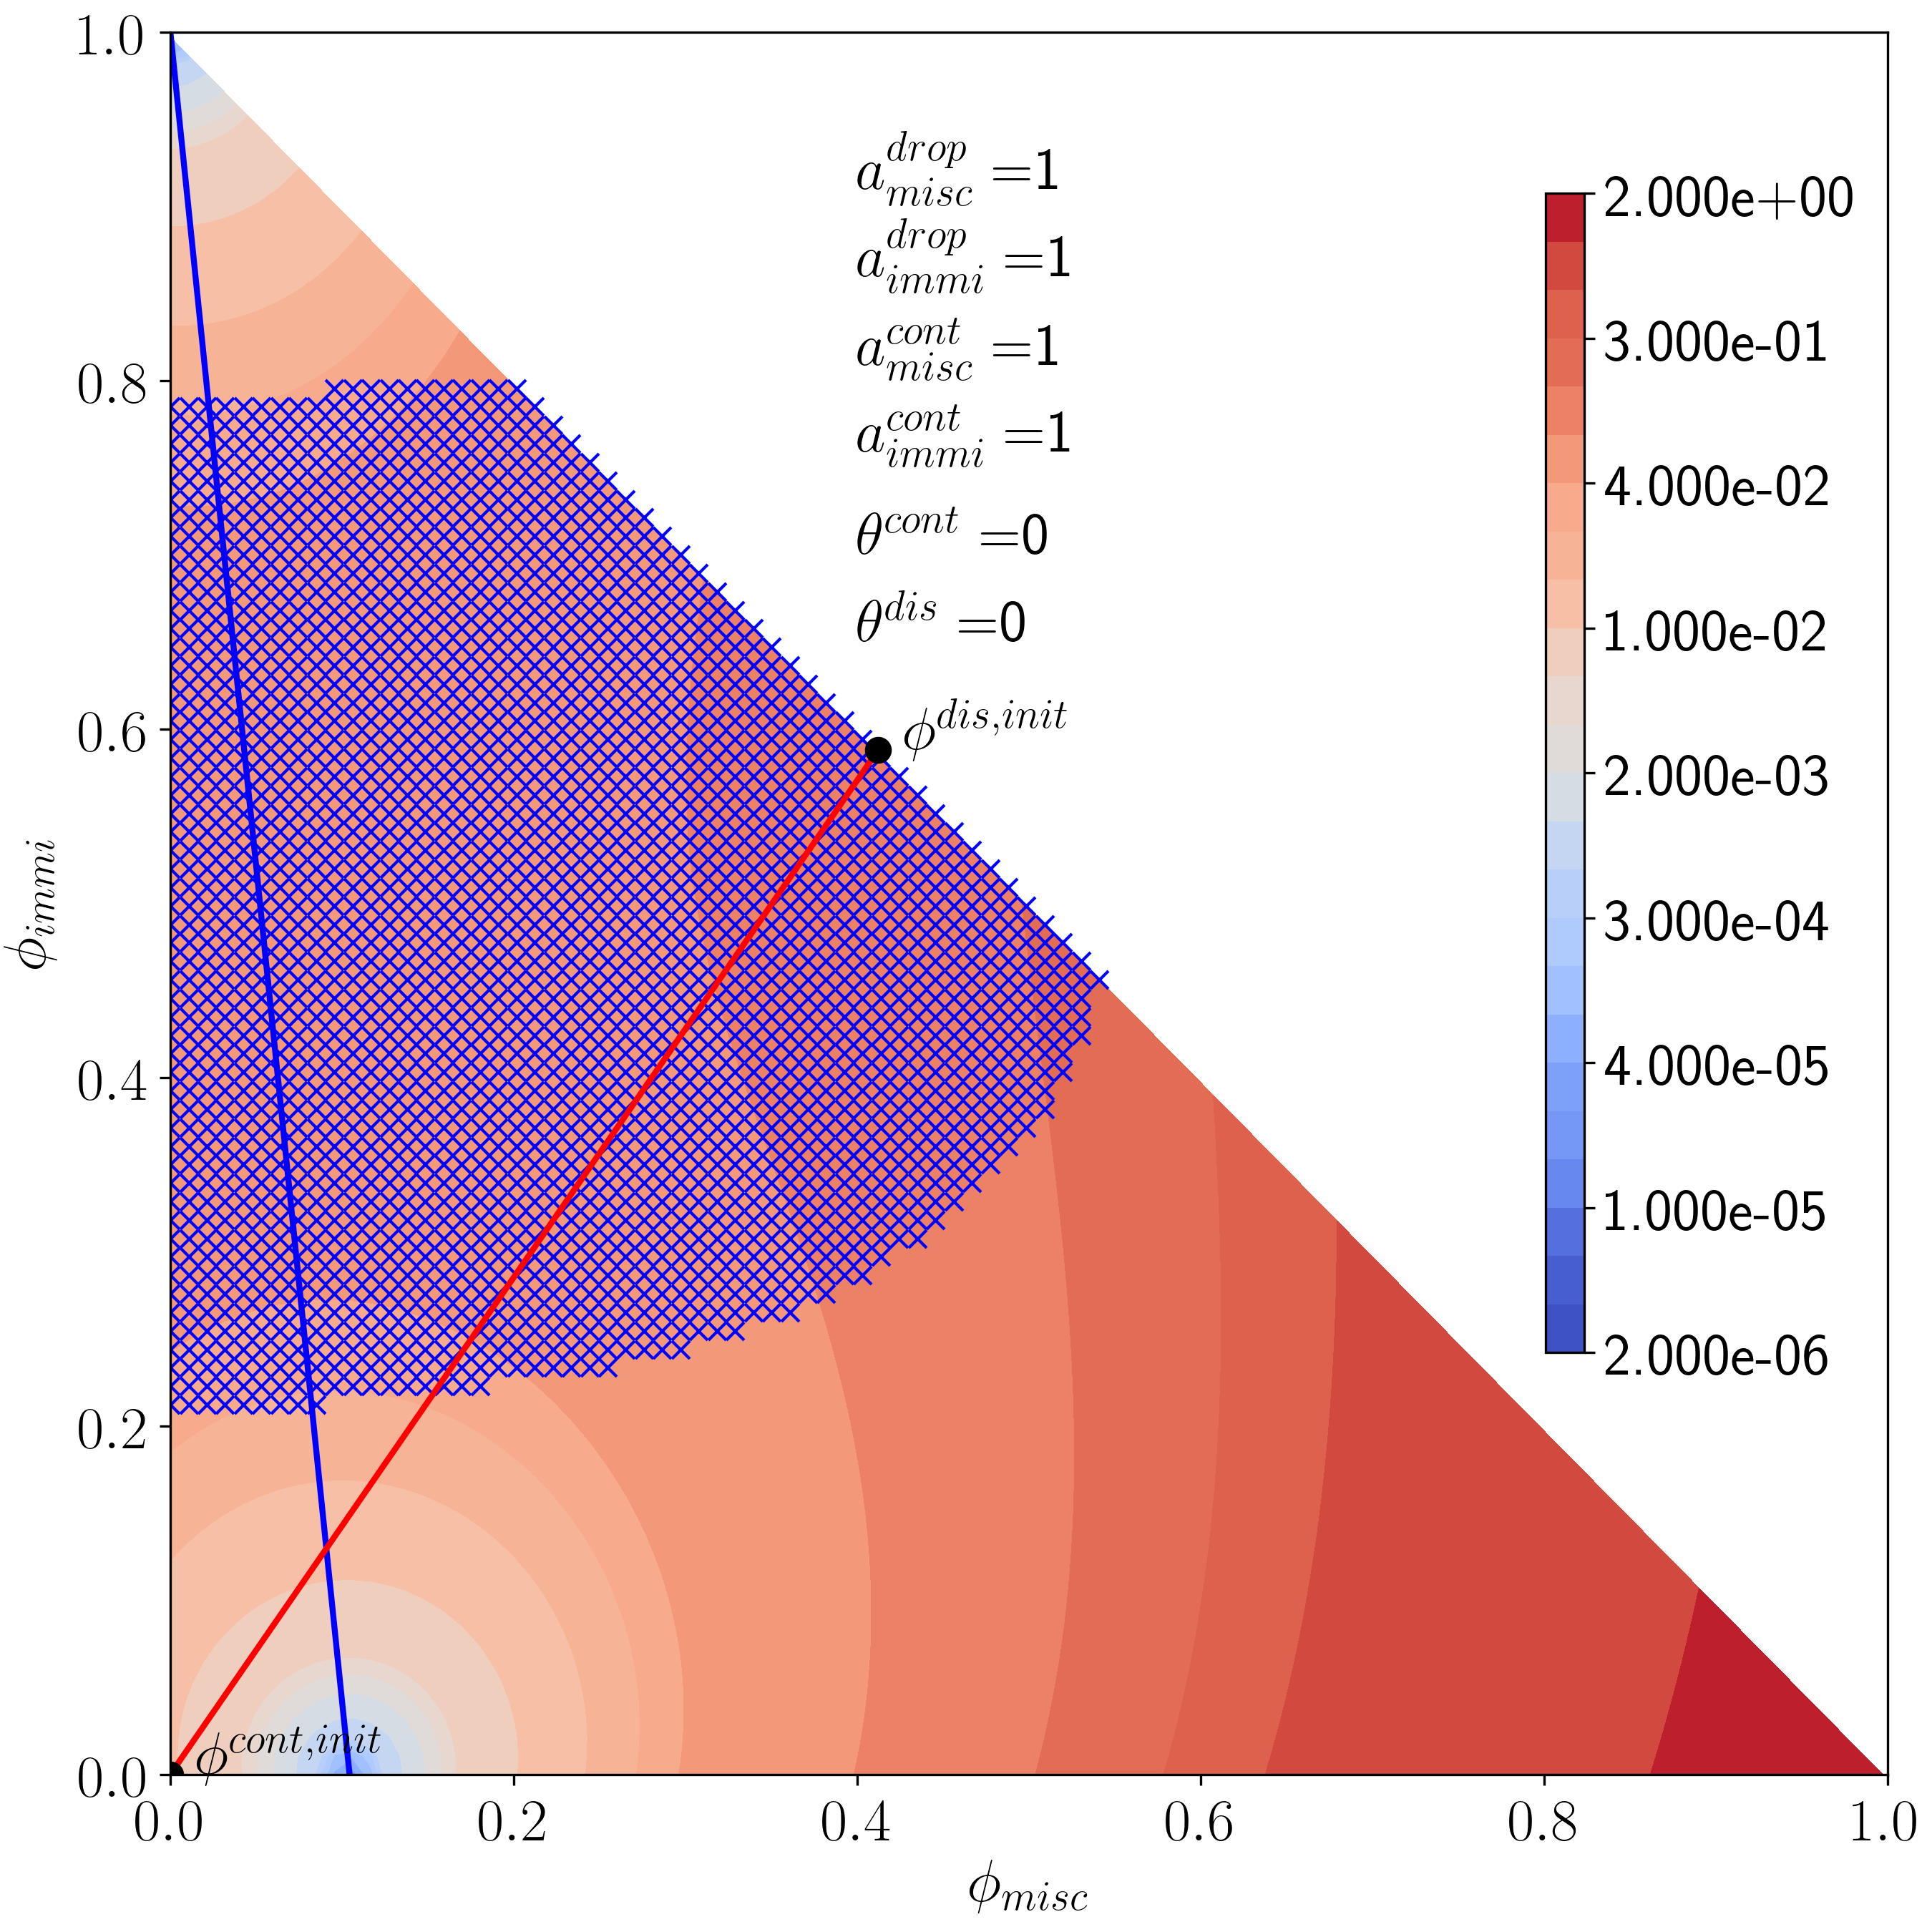
\includegraphics[width=0.4\linewidth]{figure/landscape_base.png}
 	\caption[Paysage thermodynamique]{Paysage thermodynamique, la droite bleu relie les deux  concentrations d'équilibre, la droite rouge relie les deux concentrations initiales}
 	\label{fig:landscapebase}
 \end{figure}
\vspace{-0.5cm}
 \begin{figure}[H]
 	\centering
 	\begin{subfigure}[H]{0.32\textwidth}
 		\centering
 		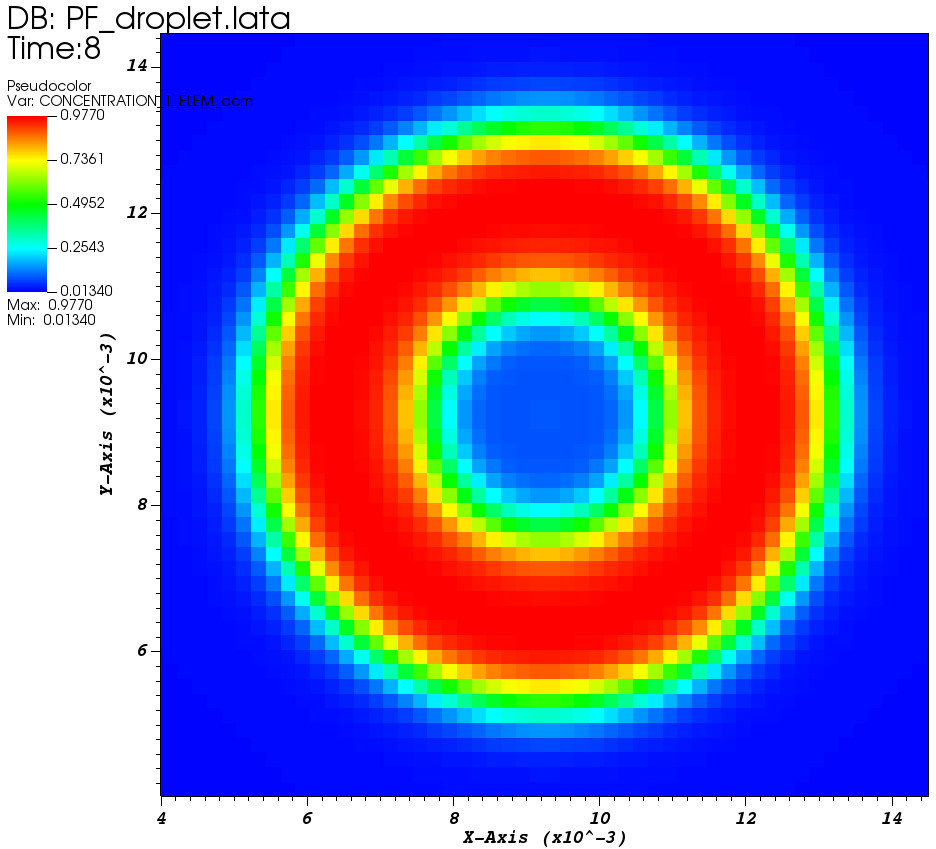
\includegraphics[width=\textwidth]{figure/paysage_base/visit0000.png}
 		\caption{Concentration immiscible}
 		\label{fig:y equals x}
 	\end{subfigure}
 	\begin{subfigure}[H]{0.32\textwidth}
 		\centering
 		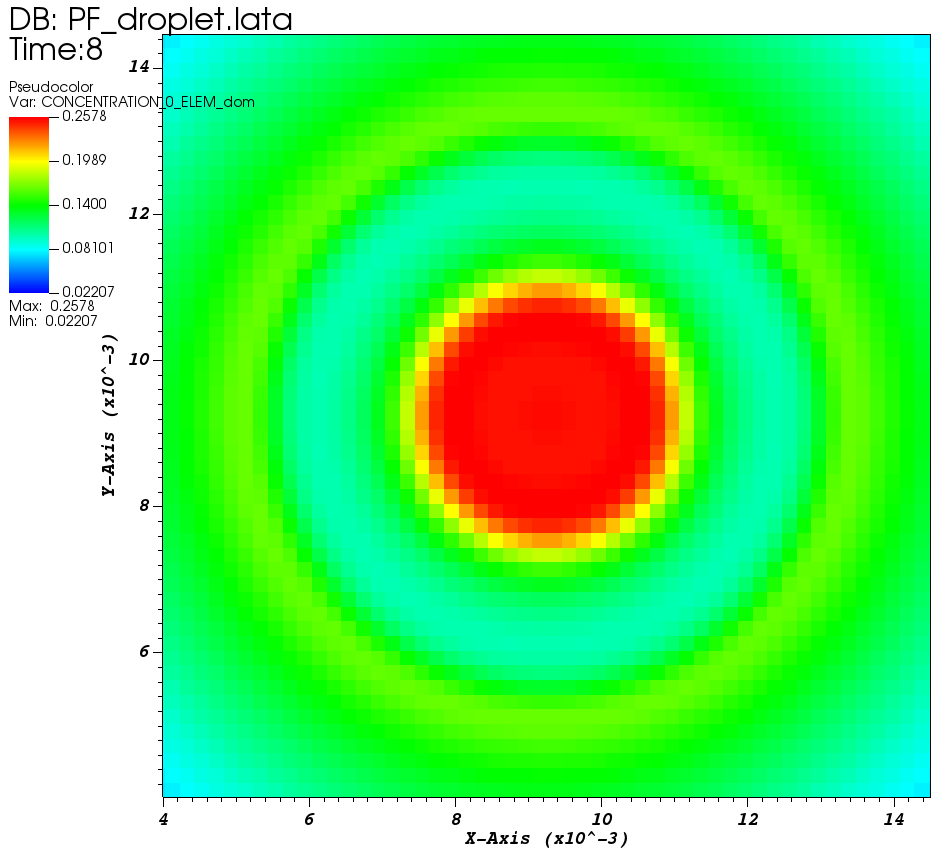
\includegraphics[width=\textwidth]{figure/paysage_base/visit0001.png}
 		\caption{Concentration miscible}
 		\label{fig:y equals x}
 	\end{subfigure}
 	\begin{subfigure}[H]{0.32\textwidth}
 		\centering
 		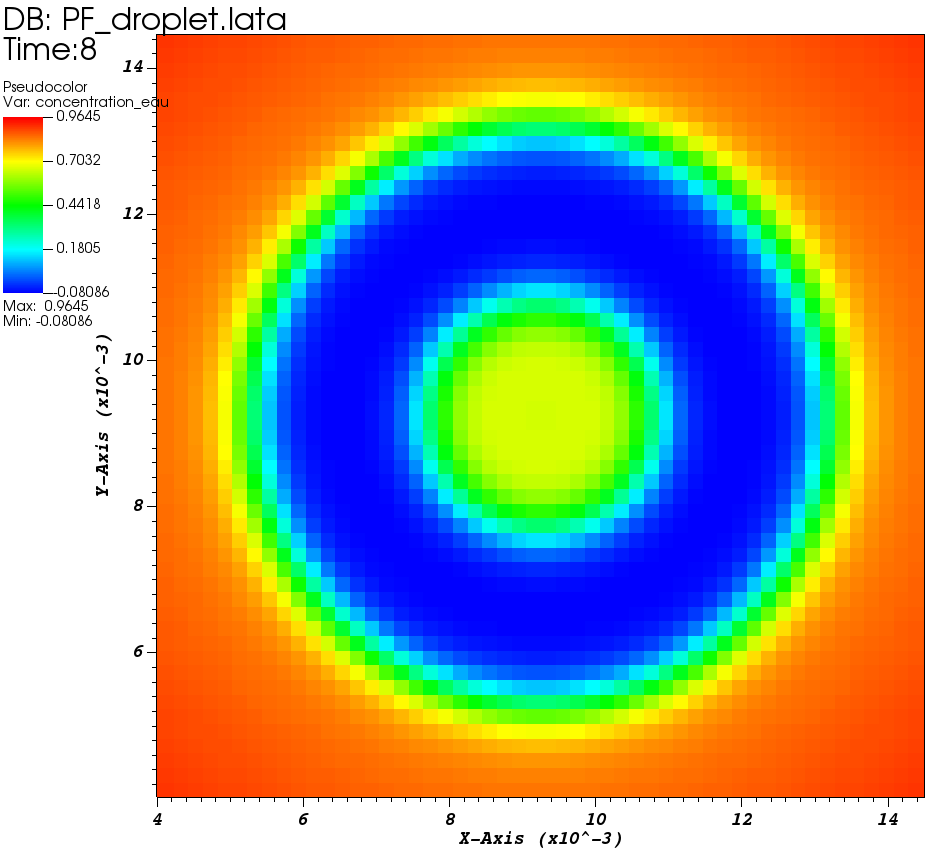
\includegraphics[width=\textwidth]{figure/paysage_base/visit0002.png}
 		\caption{Concentration eau}
 		\label{fig:y equals x}
 	\end{subfigure}
 	\caption{Séparation de phase dans la goutte}
 	\label{land_base_sep}
 \end{figure} \vspace{-0.5cm}
Sur la figure \ref{land_base_sep} on observe la présence de deux phases à l'intérieur de la goutte, une première uniquement composée de l'élément immiscible et la seconde composée d'eau et de l'élément miscible. On présente un deuxième paysage en figure \ref{fig:paysage2}
Comme expliqué précédemment ce paysage représente l'énergie libre volumique liée à l'équilibre des phases, ainsi on cherche à ce que les conditions initiales (ici aux extrémités de la droite rouge) soit hors de la zone instable et que la composition d'équilibre globale (placé a l'intersection des droites bleu et rouge) soit placée dans la lacune de miscibilité. Ainsi ce paysage semble correspondre parfaitement à ces deux critères. On souhaite également limiter l'entrée d'eau dans la goutte en régime transitoire, cette condition ce traduit par égalité entre la somme des deux compositions et l'unité. Hors ici le gradient d'énergie favorise un "chemin" différent. Pour vérifier cette présence d'eau, on considère alors un calcul statique (sans résolution des équations de Navier-Stokes) et on trace les concentrations à différents instants. On observe dès lors une importante intrusion d'eau dans la goutte dès les premiers instants, puis une séparation de phase est observable à l'intérieur de la goutte, phénomène que l'on souhaite absolument éviter.
 \begin{figure}[H]
 	\centering
 	\begin{subfigure}[H]{0.45\textwidth}
 		\centering
 		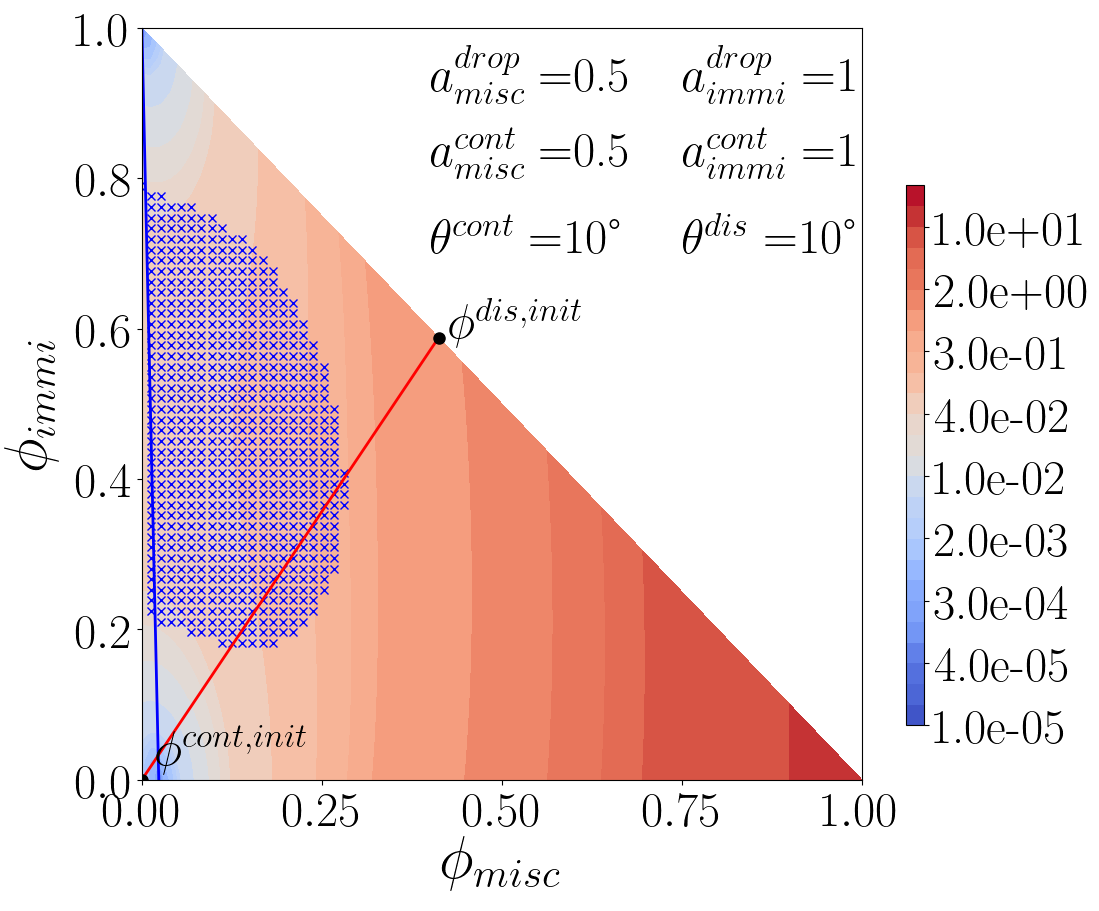
\includegraphics[width=\textwidth]{figure/paysage_neqlocal}
 		\caption{Paysage thermodynamique complet}
 		\label{fig:y equals x}
 	\end{subfigure}
 	\hfill
 	\begin{subfigure}[H]{0.45\textwidth}
 		\centering
 		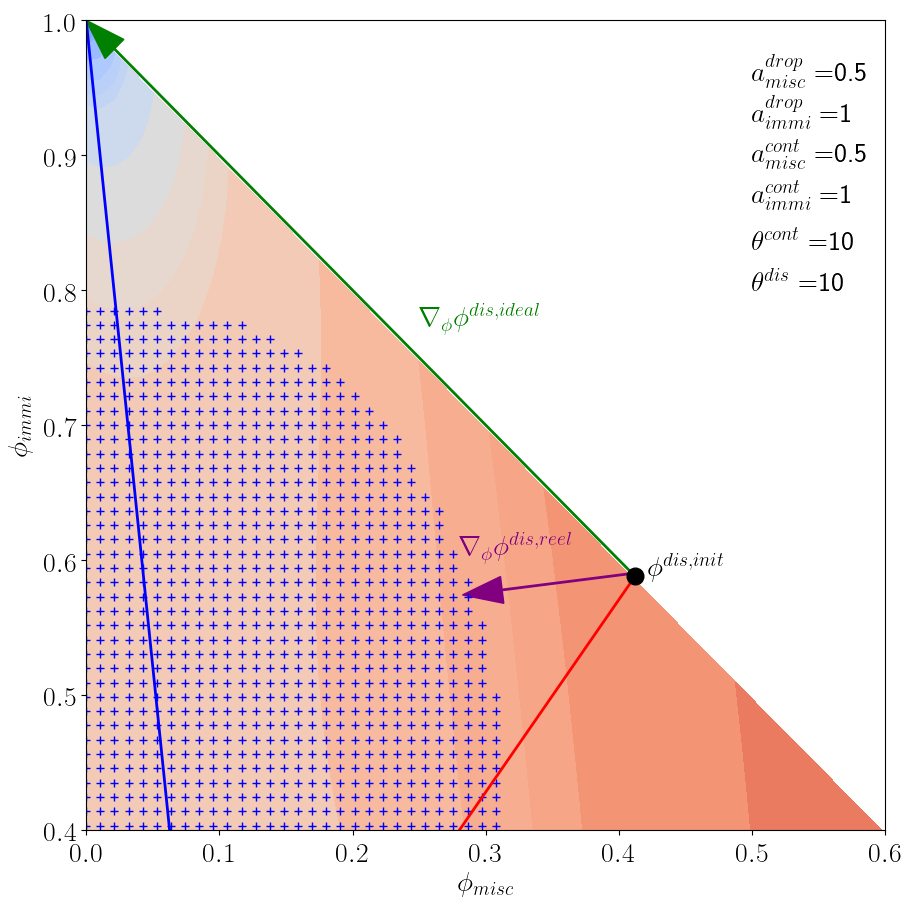
\includegraphics[width=\textwidth]{figure/direction_gradient}
 		\caption{Paysage thermodynamique partiel}
 		\label{fig:y equals x}
 	\end{subfigure}
 	\caption{Paysage thermodynamique et direction privilégiée par le système, la flèche verte représente le cas idéal sans intrusion d'eau et la flèche violette le cas associé au paysage thermodynamique, la zone bleu correspond à la zone instable}
 	\label{fig:paysage2}
 \end{figure}\vspace{-0.9cm}
 \begin{figure}[H]
 	\centering
 	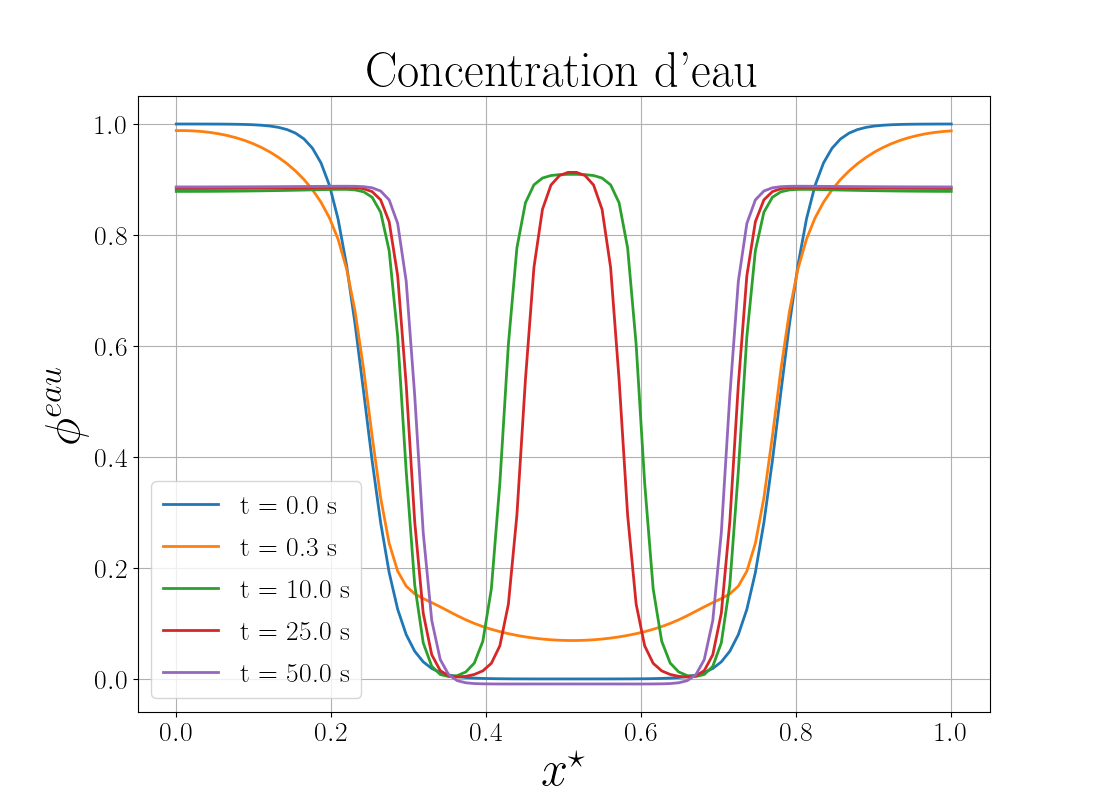
\includegraphics[width=0.7\linewidth]{figure/eau_ref}
 	\caption[Concentration d'eau dans le domaine]{Concentration d'eau dans le domaine, $x^{\star} = x / L_x$ représente une longueur adimensionnée}
 	\label{fig:eauref}
 \end{figure}\vspace{-0.7cm}
Finalement au travers de ces deux exemples, nous avons montré que pour qu'un paysage soit cohérent et potentiellement utilisable certaines conditions sont à remplir. Les critères concerne la position des conditions initiales, qui doivent être en dehors de la zone instable, un second critère concerne l'absence nécessaire de la zone instable sur le "chemin" de chacune des phases et finalement une direction initiale privilégiant une imperméabilité à l'eau dans la goutte.
\subsection{Validation d'un paysage}
Dans la suite on utilisera le paysage présenté en figure \ref{fig:thechoosenone} répondant à l'ensemble de ces critères.
\begin{figure}[H]
		\centering
		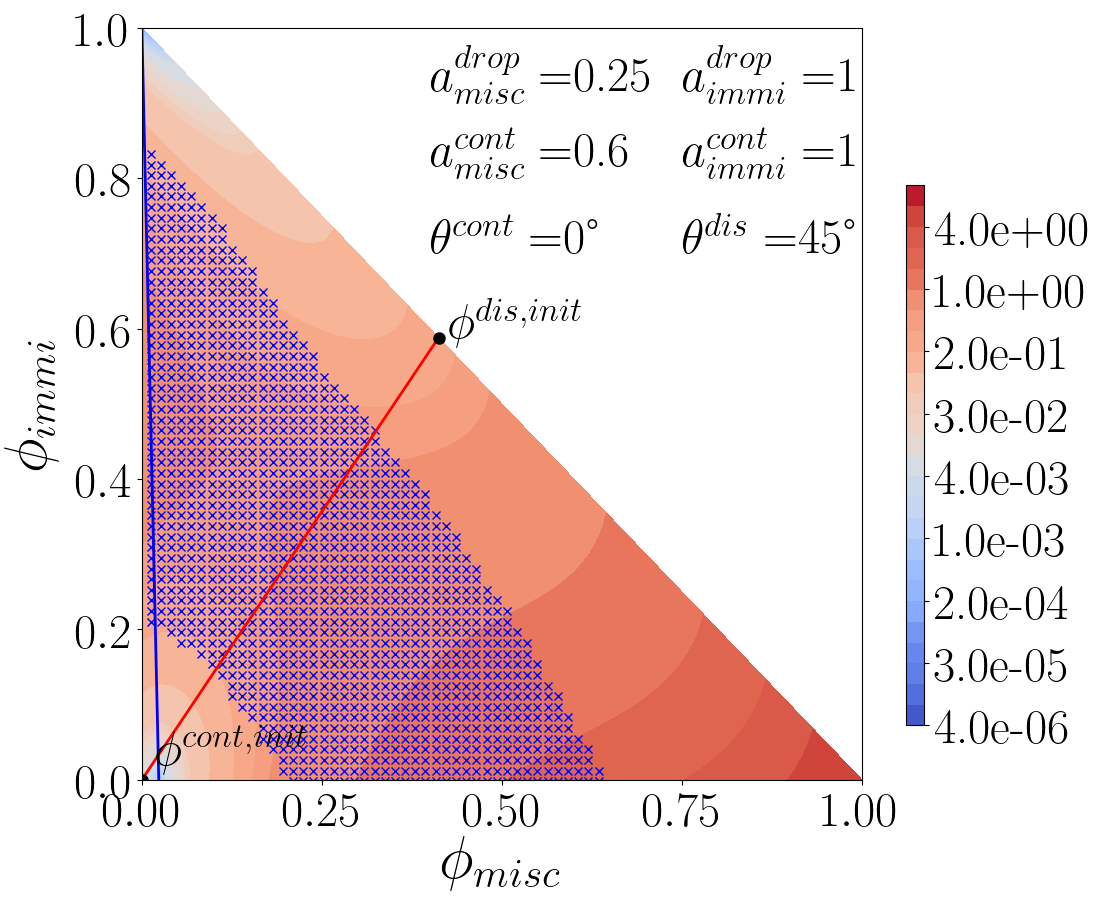
\includegraphics[width=0.45\textwidth]{figure/Paysage_ecriture1.png}
	\caption{Paysage thermodynamique choisit pour la simulation}
	\label{fig:thechoosenone}
\end{figure}

On cherche à tracer la solution stationnaire, sans couplage avec les équations de Navier-Stokes, on observe alors une non-monotonie de l'interface pour le composant miscible, de plus à l'intérieur de la goutte la concentration de composant miscible est négative et la composition d'élément immiscible est quant à elle supérieure à 1, de façon à obtenir une somme des deux concentrations égale à l'unité.
\begin{figure}[H]
	\centering
	\begin{subfigure}[H]{0.45\textwidth}
		\centering
		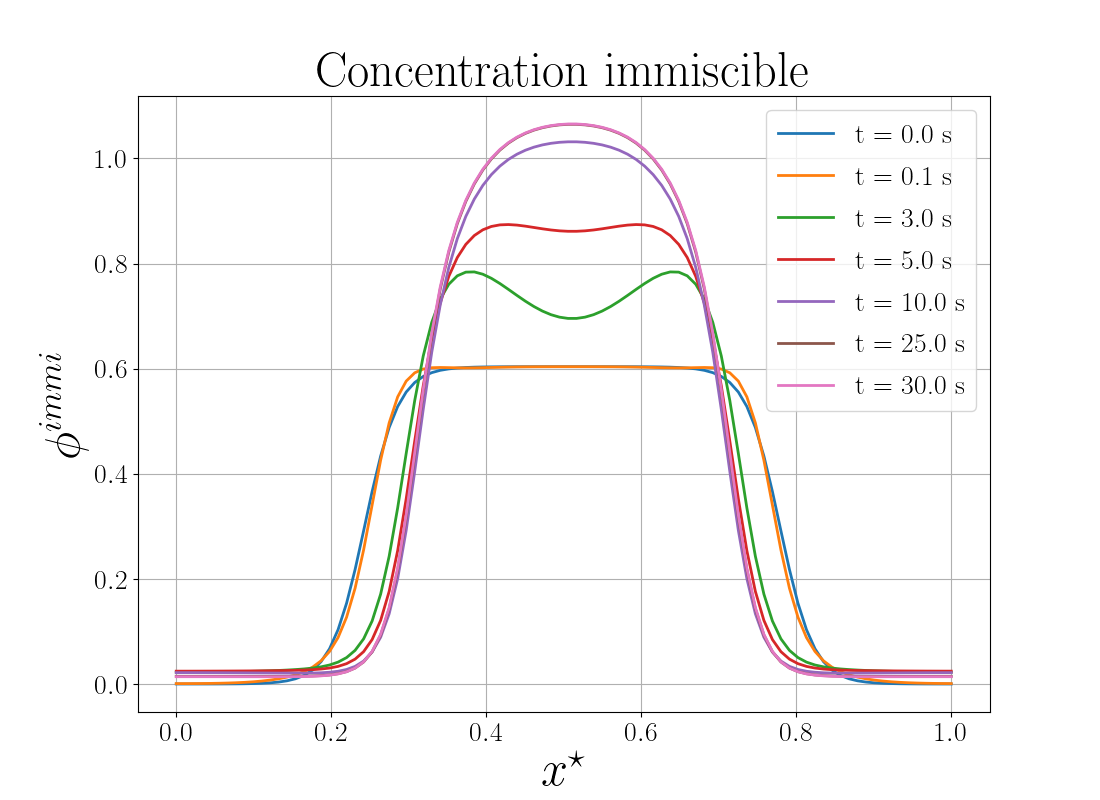
\includegraphics[width=\textwidth]{figure/nouveau_parametrage/immiscible_New_Parametrage.png}
		\caption{Concentration immiscible}
		\label{fig:y equals x}
	\end{subfigure}
	\hfill
	\begin{subfigure}[H]{0.45\textwidth}
		\centering
		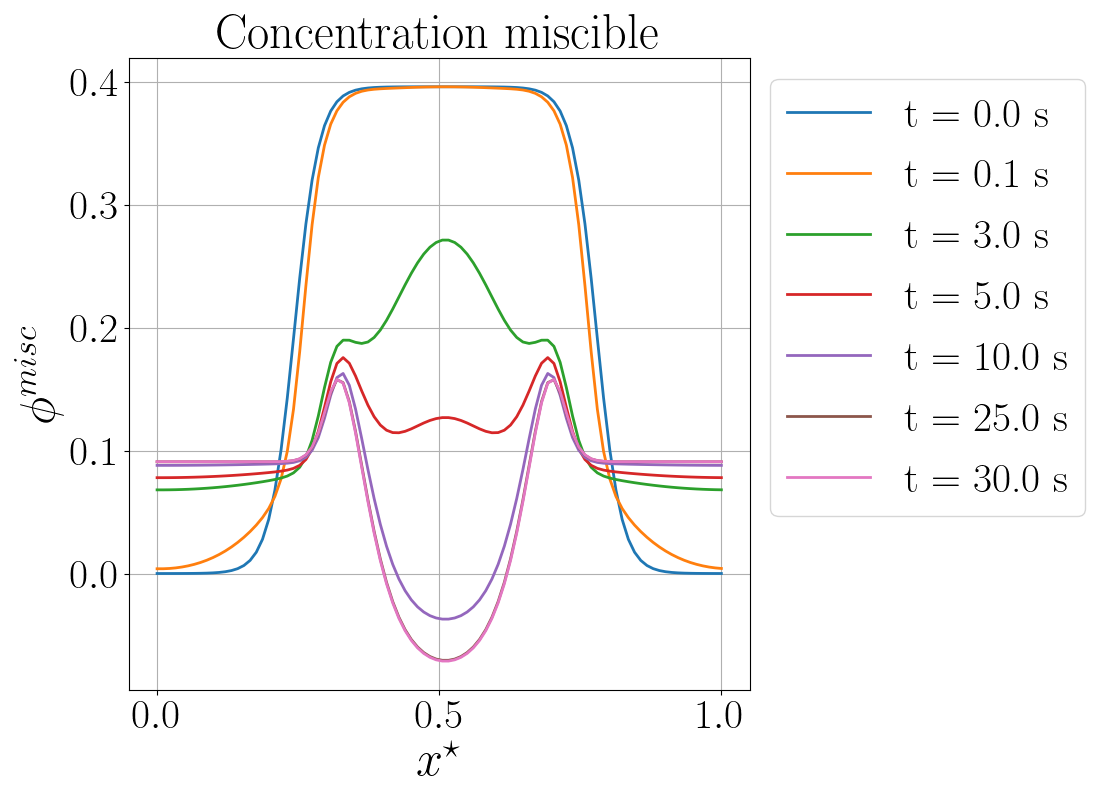
\includegraphics[width=\textwidth]{figure/nouveau_parametrage/miscible_New_Parametrage.png}
		\caption{Concentration miscible}
		\label{fig:y equals x}
	\end{subfigure}
\end{figure} \vspace{-0.8cm}
\begin{figure}[H]
	\centering
	\ContinuedFloat
	\begin{subfigure}[H]{0.45\textwidth}
		\centering
		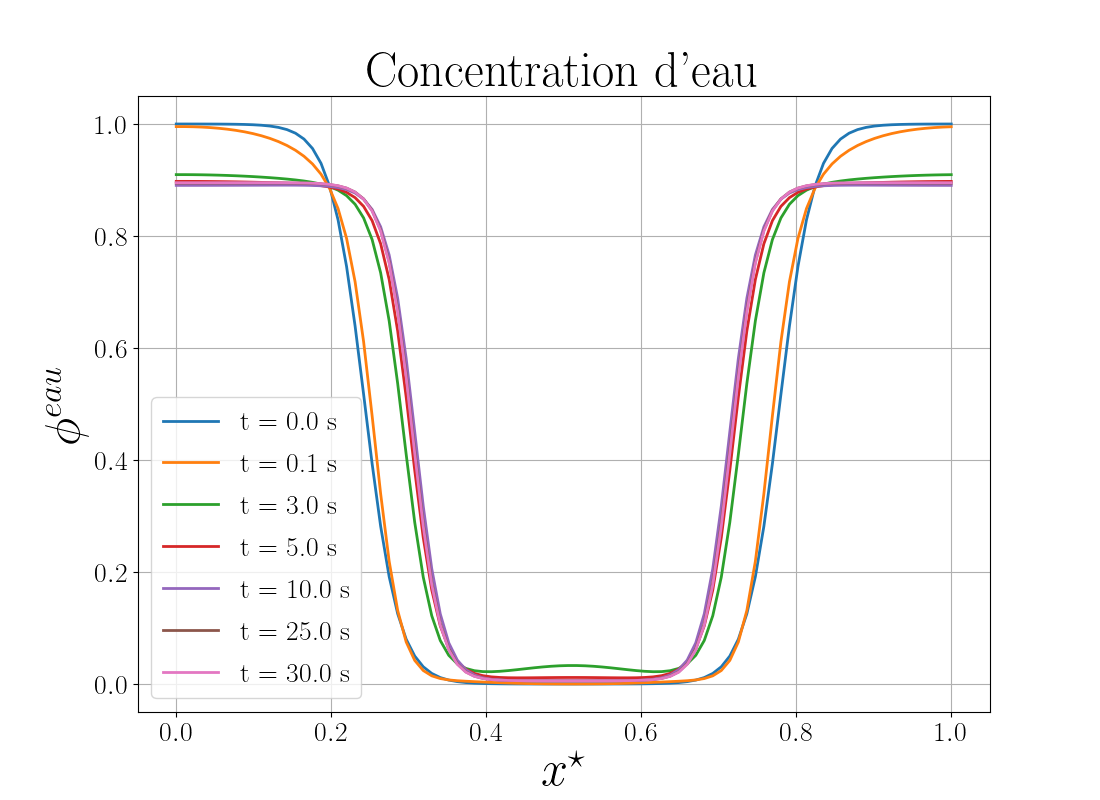
\includegraphics[width=\textwidth]{figure/nouveau_parametrage/eau_New_Parametrage.png}
		\caption{Concentration d'eau}
	\end{subfigure}
	\caption{Variation de la concentration des différents composants au cours du temps}
\end{figure}
On remarque alors une non-monotonie de l'interface. L'article \cite{rasolofomanana_diffuse-interface_2022} présente un paramétrisation du coefficient de gradient pour traiter les non monotonie d'interface, cette paramétrisation utilise la symétrie de la matrice coefficient de gradient pour la réécrire sous la forme :
\begin{equation}
\bar{\bar{\bm{\kappa}}} = \alpha \bm{R}\bm{D}\bm{R}^T
\label{eq:param_kappa}
\end{equation}
avec : $\bm{R}$ une matrice de rotation et $\bm{D}$ une matrice diagonale de la forme :
\begin{equation}
\bm{R} =    \begin{pmatrix} 
\cos\varphi & -\sin\varphi \\ 
\sin\varphi				&  \cos\varphi
\end{pmatrix}
\end{equation}
\begin{equation}
	\bm{D}(d) =    \begin{pmatrix} 
	2 & 0 \\ 
	0 & d
	\end{pmatrix} 
\end{equation}
La cohérence avec le système binaire est assurée par le coefficient $\alpha$ obtenu tel que :
\begin{equation}
\alpha = \frac{\kappa^{bin}}{2\cos^2\varphi + d \sin^2\varphi}
\end{equation}
On présente les différents résultats issus de la paramétrisation du coefficient de gradient : 
\begin{figure}[H]
		\centering
		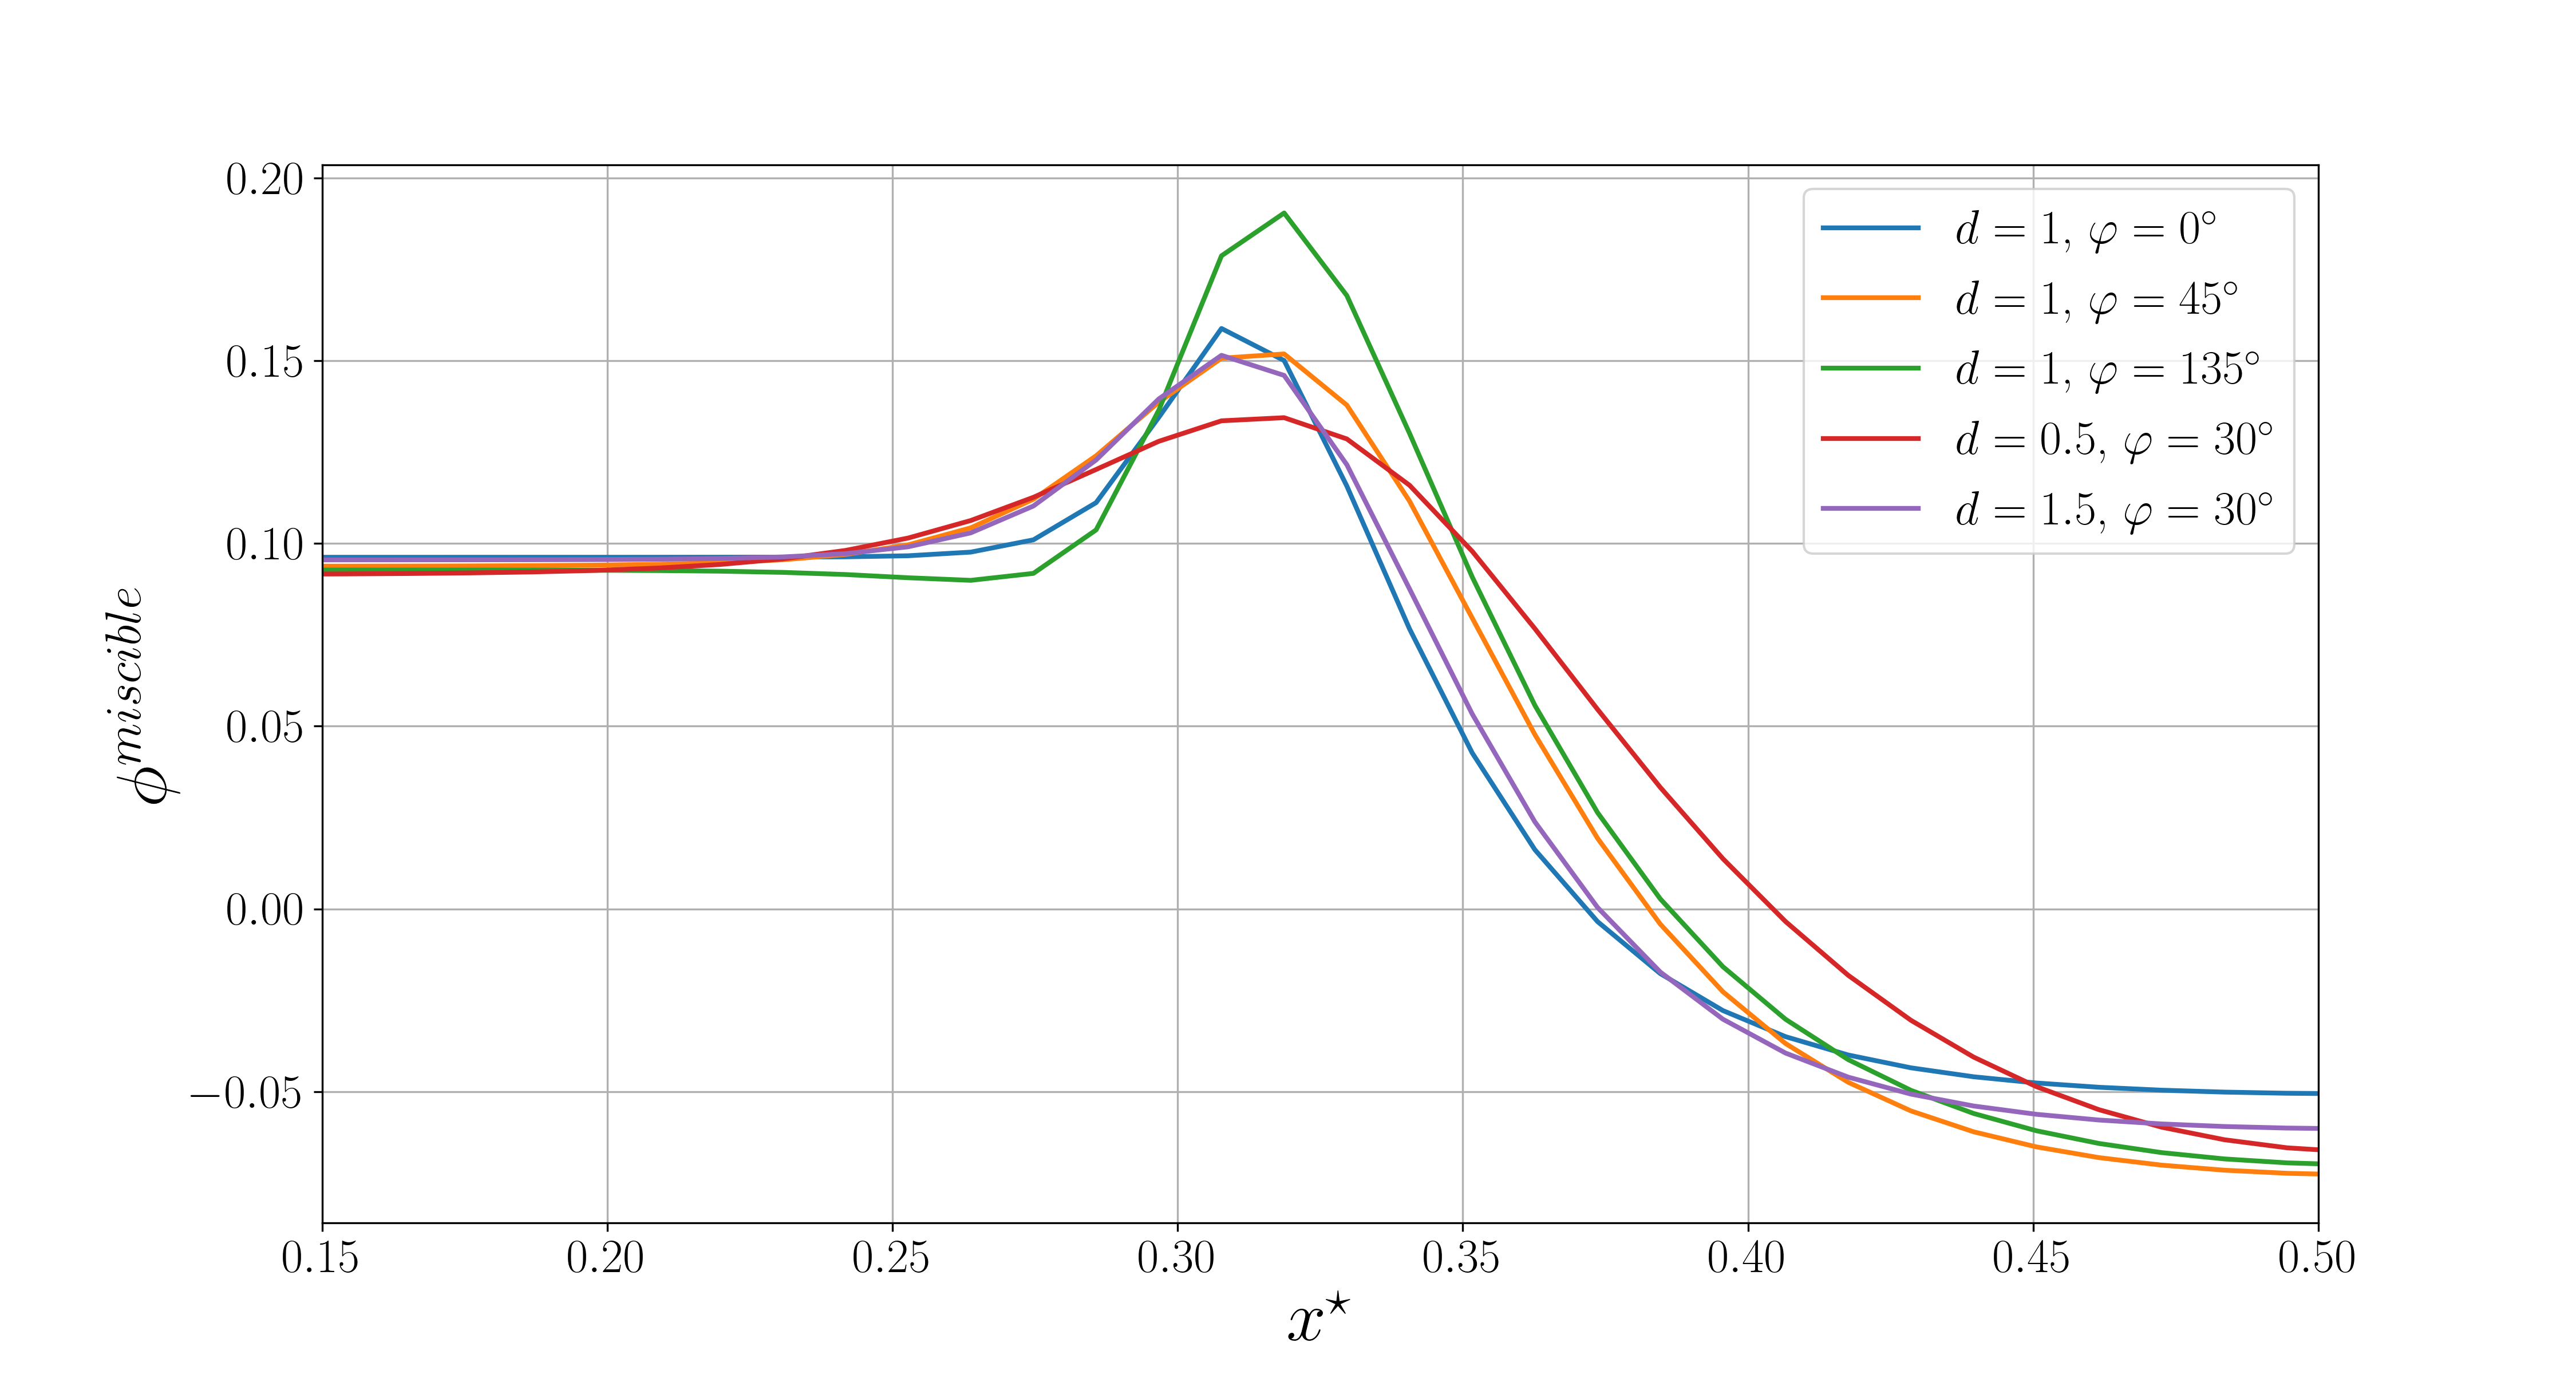
\includegraphics[width=0.7\textwidth]{figure/ProfInterfStatio2.png}
		\caption{Profils de l'interface pour différents paramétrages du coefficient de gradient}
\end{figure}

